\section{Introduction}\label{sec:introduction}


This paper considers two classical optimization problems: the \emph{offline $k$-server} problem and the \emph{minimum-cost bipartite matching} problem in geometric settings. %We begin by introducing these problems.
%\todo{Needs to be updated.} Many service providers such as taxi, package, and grocery delivery offer to provide their services at a requested time. In such cases, each service request is specified by a delivery location and a service time. Given a sequence $\requests$ of request locations ordered by the request time and $k$ service providers, $\requests$ is partitioned into $k$ subsequences and assigned to each of the $k$ service providers. Each service provider then serves the requests in their subsequence in increasing order of the request time. Motivated by such applications, we consider the problem of finding the cheapest set of routes for $k$ service providers to serve the $n$ requests in the sequence. 

 
\myparagraph{Offline $k$-server problem and its variant.} Consider a sequence of requests $\varsigma = \langle r_1,\ldots, r_m \rangle$ in a metric space equipped with the cost function $\distance{\cdot}{\cdot}$. The cost of a single server \emph{servicing} the requests in $\varsigma$ is the sum of the distances between every consecutive pair of points in the sequence, i.e.,  $\seqcost(\varsigma)=\sum_{i=1}^{m-1} \distance{r_i}{r_{i+1}}$. Given a sequence $\requests = \langle r_1,\ldots r_n\rangle$ of $n$ requests and an integer $1 \le k \le n$, the \emph{$k$-sequence partitioning problem} (or simply the $k$-SP problem) requires partitioning the requests in $\requests$ into $k$ subsequences $\varsigma_1, \ldots, \varsigma_k$ so that $\sum_{i=1}^{k}\seqcost(\varsigma_i)$ is minimized. The optimal solution for the $k$-sequence partitioning problem is the cheapest way for $k$ servers to service all of the requests in $\requests$. 
We also consider a variant: the \emph{$k$-sequence partitioning with initial locations problem} (or the $k$-SPI problem). Here,
 in addition to the requests $\requests$, we are also given the initial locations $\eta=\langle s_1,\ldots, s_k\rangle$ for the $k$ servers. The objective of this problem is to partition $\requests' = \eta \requests$ into $k$ subsequences $\varsigma_1,\ldots, \varsigma_k$ so that the initial location $s_j$ of server $j$ appears in the first element of the subsequence $\varsigma_j$ and the cost $\sum_{i=1}^{k}\seqcost(\varsigma_k)$ is minimized. 
The optimal solution to the $k$-SPI problem is the offline optimal solution to the well-known $k$-server problem. 

We assume that the requests in $\requests$ and the initial locations in $\eta$ are scaled and translated so that they are contained inside the unit hypercube $[0,1]^d$. Such scaling and translation do not impact the optimal solutions for the $k$-SP and $k$-SPI problems. We define the diameter $\mathrm{Diam}(\requests)$ to be the largest distance between any two request locations in $\requests$ and the \emph{closest pair distance}, denoted by $\mathrm{CP}(\requests)$, to be the smallest non-zero distance between any two requests in $\requests$. The \emph{spread}, denoted by $\Delta$, is the ratio of the diameter to the closest-pair distance, i.e., $\Delta=\mathrm{Diam}(\requests)/\mathrm{CP}(\requests)$. 

\myparagraph{Minimum-cost bipartite matching.} Consider a weighted bipartite graph $G(A\cup B, E\subseteq A\times B)$, where each edge between $u$ and $v$ is assigned a real-valued cost. Let $n:=\min\{|A|, |B|\}$. A \emph{matching} of size $t\le n$, or simply a \emph{$t$-matching}, is a set of $t$ edges in $G$ that are vertex-disjoint. The \emph{cost} of any matching $M$ is the sum of the costs of its edges. Given a parameter $t \le n$, the \emph{minimum-cost bipartite $t$-matching} problem seeks to find a $t$-matching with a minimum cost. %When $t=n$, the problem is called the \emph{minimum-cost maximum bipartite matching} problem. 
When $|A|=|B|=n$, a matching of size $n$ is called a \emph{perfect matching}. When $A$ and $B$ are $d$-dimensional point sets and the cost of any edge between $a \in A$ and $b \in B$ is the $\ell_p$ distance $\|a-b\|_p$, the problem of finding the minimum-cost bipartite $t$-matching is also called the (partial) \emph{geometric bipartite matching problem}. 


%Given two $d$-dimensional points $a$ and $b$, let the $\ell_p$ cost between $a$ and $b$ be $\|a-b\|_p$. In the \emph{minimum-cost bipartite matching (MCBM) problem} with $\ell_p$ costs, or the \emph{geometric bipartite matching}, we are given two sets $A$ and $B$ of $d$-dimensional points with $n=\min\{|A|, |B|\}$. Consider a bipartite graph with $G(A\cup B, E\subseteq A\times B)$ where an edge between $a$ and $b$ has a cost of $\|a-b\|_p$. A \emph{matching} of size $t\le n$ is a set of $t$ vertex disjoint edges in $G$ and a perfect matching in $G$ is any matching of size $n$. Given a parameter $t \le n$, the \emph{minimum-cost $t$-partial matching} problem computes a minimum-cost matching of size $t$. Any point $u\in A\cup B$ that is not incident on any matching edges in $M$ is called a \emph{free} point. The geometric bipartite matching on a complete graph with $E=A\times B$ is a classic geometric optimization problem that has been extensively studied in computational geometry. 


\myparagraph{Relating the two problems.}
\citet{chrobak1991new} established a reduction from the minimum-cost bipartite $t$-matching problem to the $k$-SPI problem.
\begin{lemma}\cite[Theorem 11]{chrobak1991new}
\label{lem:spimatch}
Any algorithm that computes an optimal solution to the $n$-SPI in an arbitrary metric space in $T(n)$ time can also find, in $T(n)+O(n^2)$ time, a minimum-cost perfect matching in any complete bipartite graph with real-valued costs.
\end{lemma}

We strengthen the connection between the two problems by showing a reduction in the reverse direction, i.e., we reduce the $k$-SP (resp. $k$-SPI) problem to the minimum-cost bipartite $t$-matching problem.
Given an input sequence $\requests$ of requests to the $k$-SP problem, we construct a bipartite graph $\mathcal{G}_{\requests}$ with a vertex set $A\cup B$ and a set of edges $\mathcal{E}$ as follows. 
{\it Vertex Set:} For each request $r_i$, we create a vertex $b_i$ (resp. $a_i$) in $B$ (resp. $A$) and designate it as the \emph{entry} (resp. \emph{exit}) gate for request $r_i$. 
{\it Edge Set:} The exit gate $a_i$ of request $r_i$ is connected to the entry gate $b_j$ of every subsequent request $r_j$ with $j > i$ with an edge. The cost of this edge is $\distance{a_i}{b_j}=\|r_i-r_j\|_p$. 
It is easy to see that a minimum-cost $(n-k)$-matching $M$ in $\mathcal{G}_\requests$ can be used to find an optimal solution to the $k$-SP problem. See Figure~\ref{fig:problem}. 

For the $k$-SPI problem, for each server $j$, we add a vertex $a^j$ at the initial location $s_j$ to $A$ and connect $a^j$ to the entry gate $b_i$ of every request $r_i$ in $\requests$. The cost of this edge is $\distance{a^j}{b_i}=\|s_j-b_i\|_p$. A minimum-cost $n$-matching in this graph can be converted to an optimal solution for the $k$-SPI problem. The formal proof of correctness for both these reductions is presented in Appendix~\ref{sec:background}.

A different reduction from $k$-SP and $k$-SPI problems to the minimum-cost flow problem has been presented in previous works~\cite{chrobak1991new, rudec2009fast, rudec2013new}, leading to the development of $O(n^2k)$ time algorithm. However, unlike our reduction, their approach generates instances that include edges whose costs are $-\infty$ and fails to maintain the metric properties of costs.
\begin{figure}
    \centering
    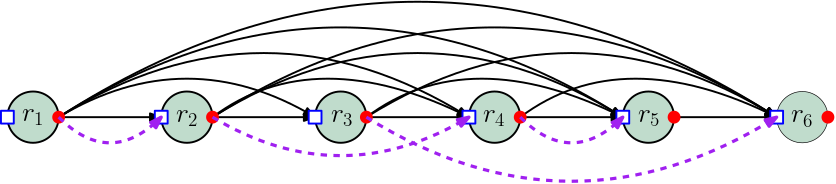
\includegraphics[width=0.9\textwidth]{figures/problem-line5.png}
    \caption{The graph $\mcG_\requests$ constructed for $\requests=\langle r_1, r_2, \ldots, r_6\rangle$. The vertex set $A$ (red disks) and $B$ (blue squares) represent the exit and entry gates of each request, and the purple dashed lines show an $(n-2)$-partial matching on $\mcG_\requests$ representing a $2$-partitioning $\langle r_1, r_2, r_4, r_5\rangle$ and $\langle r_3, r_6\rangle$.}
    \label{fig:problem}
\end{figure}


% Similarly, given an input $\requests'=\eta\requests$ to the $k$-SPI problem, we construct a graph $\mathcal{G}_{\requests'}$ as follows.
% {\it Vertex Set:} For any server $j$ and its initial location $s_j$, we create a single vertex $a^j$ 
% % referred to as the exit gate 
% and add it to the set $A$. For each request $r_i$ in $\requests$, we create a vertex $b_i$ (resp. $a_i$) in $B$ (resp. $A$) and  refer to it as the entry (resp. exit) gate for $r_i$. 
% {\it Edge Set:} We connect every $a^j$ to all points $b_i\in B$ with an edge and assign it a cost $\distance{a^j}{b_i}:=\|s_j-r_i\|_p^q$. For any $r_i$ and every $j > i$, we connect the exit gate $a_i$ to the entry gate $b_j$ and assign it a cost $\distance{a_i}{b_j}:=\|r_i-r_j\|_p^q$. 
% Like in the case of $k$-SP, we show that a minimum-cost matching of size $n$ in $\mathcal{G}_{\requests'}$ can be converted to an optimal solution to the $k$-SPI problem.

\begin{lemma}\label{lemma:matching-reduction} 
An optimal solution for an instance $\requests$ (resp. $\requests'$) of $k$-SP (resp. $k$-SPI)  problem can be found by computing a minimum-cost matching of size $n-k$ (resp. $n$) in $\mathcal{G}_{\requests}$ (resp. $\mathcal{G}_{\requests'}$).
\end{lemma}


%When $A$ and $B$ are $d$-dimensional points and the costs are $\ell_p$, one can adapt geometric matching algorithms to compute the optimal solution to $\mathcal{G}_{\requests}$ in $\tilde{O}(n^2\Phi(n))$ time; here $\Phi(n)$ is the query/update time of a dynamic weighted nearest neighbor data structure\footnote{In this paper, we present an improved algorithm with a running time of $\tilde{O}(nk\Phi(n))$. See Section~\ref{sec:nk-algod}.}. We next present a reduction from the bipartite matching problem to the $k$-SPI problem,  showing that improving the quadratic bound may be challenging. 

Finally, we extend the reduction~\citet{chrobak1991new} to geometric settings and provide a reduction from the geometric minimum-cost matching problem under the $\ell_1$-norm to the geometric version of the $n$-SPI problem. 
This reduction, however, creates an instance of the $n$-SPI problem with a spread of $3^n$ (See Appendix~\ref{sec:reduction} for details). Lemma~\ref{lemma:kSPI_reduction} follows directly from this reduction.  %Lemma~\ref{lemma:kSPI_reduction}, we reduce the minimum-cost bipartite matching problem in the geometric settings to the $n$-SPI problem. 

%We show that any algorithm that solves the $n$-SPI under $\ell_1$ costs can also be used to solve geometric bipartite matching under $\ell_1$ costs. We convert an instance of the geometric bipartite matching on $d$-dimensional points $A=\{a_1,\ldots, a_n\}$ and $B=\{b_1,\ldots, b_n\}$ with a diameter of $\diam$ into a $(d+1)$-dimensional instance of the $n$-SPI problem as follows: We add $0$ as the $(d+1)^{st}$ coordinate for every point in $B$ and for each point $a_i \in A$, we add $3^{n-i+1}\diam$ as its $(d+1)^{st}$ coordinate. We create an instance of $n$-SPI by simply setting points of $B$ as the initial locations of the $n$ servers and $\langle a_1,\ldots, a_n\rangle$ as the request sequence.  See Figure~\ref{fig:EBM-intro}. We show that the optimal solution to the $n$-SPI problem on $\sigma'=\eta\sigma$ corresponds to the optimal bipartite matching between $A$ and $B$ (Appendix~\ref{sec:reduction}), leading to the following lemma.

%\begin{figure}
%    \centering
%    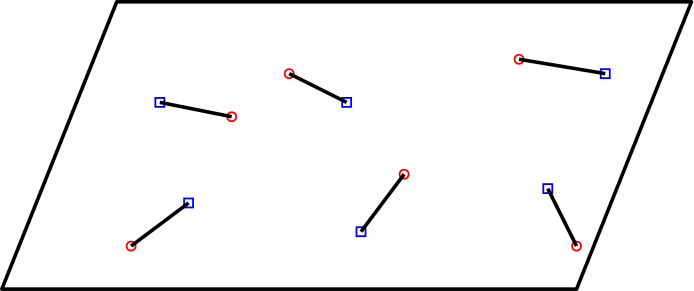
\includegraphics[width=0.45\textwidth]{figures/reduction-EBM-2.png}
%    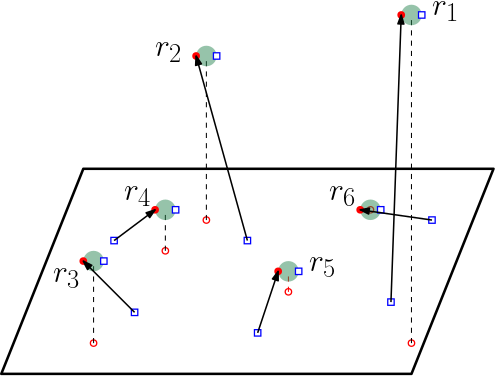
\includegraphics[width=0.45\textwidth]{figures/reduction-EBM3-4.png}
%    \caption{(left) the point set $A$ (red points) and $B$ (blue points) and a minimum-cost bipartite matching between them, (right) the instance of $n$-SPI problem we construct from $A\cup B$.}
%    \label{fig:EBM-intro}
%\end{figure}



\begin{lemma}\label{lemma:kSPI_reduction}
Any algorithm that can solve the $d$-dimensional $n$-SPI problem under the $\ell_1$ costs in $T(n)$ time can also be used to solve an instance of minimum-cost bipartite matching under the $\ell_1$ costs on a complete graph in $T(n)$ time.
\end{lemma} 


%Obtaining sub-quadratic algorithms for the geometric bipartite matching is a major open question in computational geometry. Therefore, from Lemma~\ref{lemma:kSPI_reduction}, obtaining sub-quadratic bounds for all values of $k$ is challenging.








\myparagraph{Related work.}
For a graph with $m$ edges and $n$ vertices, the classical Hungarian algorithm computes a minimum-cost $t$-matching for all values of $0\le t\le n$~\cite{kuhn1955hungarian, phatak2022computing}. The algorithm begins with an empty matching $M$, and in each iteration $i$, updates a minimum-cost $(i-1)$-matching to a minimum-cost $i$-matching in $O(m+n\log n)$ time by finding a \emph{minimum net-cost augmenting path}, i.e., an augmenting path that increases the matching cost by the smallest value. The overall execution time of the Hungarian algorithm is $O(nm+n^2\log n)$, or $O(n^3)$ when $m = \Theta(n^2)$.  
Despite substantial efforts, this remains the most efficient algorithm for the problem. Notable exceptions include specialized cases, such as graphs with small vertex separators~\cite{lipton1980applications} as well as graphs where the edge weights are integers~\cite{chen2022maximum,gt_sjc89,gt_jacm91}. 
%For graphs with real-valued edge weights, these algorithms only provide an additive approximation.


In geometric settings, Vaidya showed that each iteration of the Hungarian algorithm can be implemented in $\tilde{O}(n\Phi(n))$ time, where $\Phi(n)$ represents the query/update time of a dynamic weighted nearest neighbor (DWNN) data structure with respect to the edge costs. Thus, the minimum-cost $t$-matching can be computed in $O(n^2 \Phi(n))$ time, which is sub-cubic in $n$ provided $\Phi(n)$ is sub-linear.  For instance, for the $\ell_1$ norm and $d$ dimensions, $\Phi(n)=O(\log^d n)$~\cite{vaidya1989geometry} and for the $\ell_2$ norm and $2$ dimensions, $\Phi(n)=\log^{O(1)}n$~\cite{kaplan2020dynamic}. In these cases, the Hungarian algorithm can be implemented in near-quadratic time.  

The design of algorithms that compute a minimum-cost matching with a sub-quadratic number of queries to a DWNN data structure remains an important open problem in computational geometry. There are three notable exceptions to this. First, for points with integer coordinates and the $\ell_1$ and $\ell_\infty$ norms, the edge costs are integers. Using this fact,~\citet{ra_soda12} adapted an existing cost-scaling-based graph algorithm~\cite{gt_sjc89} and presented an algorithm that executes in $\tilde{O}(n^{3/2}\Phi(n))$ time. Second,~\citet{s_socg13} extended this result to two-dimensional point sets with integer coordinates and the $\ell_2$ costs. Their result, however, relies on the points being planar as well as the edge costs being the square root of integers and does not extend to $d$-dimensional points with real-valued coordinates.
%More recently, Gattani \textit{et al.}~\cite{gattani2023robust} presented a divide-and-conquer algorithm to compute the optimal minimum-cost matching.  The worst-case execution time of their algorithm is $\tilde{O}(n^2\Phi(n)\log\Delta)$. However, when points $A$ is a random subset of a set $U$ of $2n$ points inside the unit square and $B=U\setminus A$, their algorithm computes the optimal matching under the Euclidean costs in $\tilde{O}(n^{7/4}\Phi(n)\log \Delta))$ time.  Here, $\Delta$ is the spread of the point sets $A$ and $B$, which is the ratio of the largest to the smallest pairwise distances in $A\cup B$. \footnote{The efficiency of GRS algorithm was originally analyzed for the case where $A$ and $B$ are points drawn from an unknown distribution $\mu$. Their analysis, however, can be easily extended to the case of random subsets for an arbitrary set $U$ of $2n$ points.}.
Third, \citet{gattani2023robust} presented a divide-and-conquer algorithm (GRS algorithm) to compute a minimum-cost perfect matching. The worst-case execution time of their algorithm is $\tilde{O}(n^2\Phi(n)\log\Delta)$; here, $\Delta$ is the spread of the point sets $A$ and $B$.
For \emph{stochastic} points sampled from an unknown distribution $\mu$ in two dimensions, the algorithm finds the minimum-cost matching in $\tilde{O}(n^{7/4}\Phi(n)\log \Delta))$ time in expectation. 

\begin{figure}
    \centering
    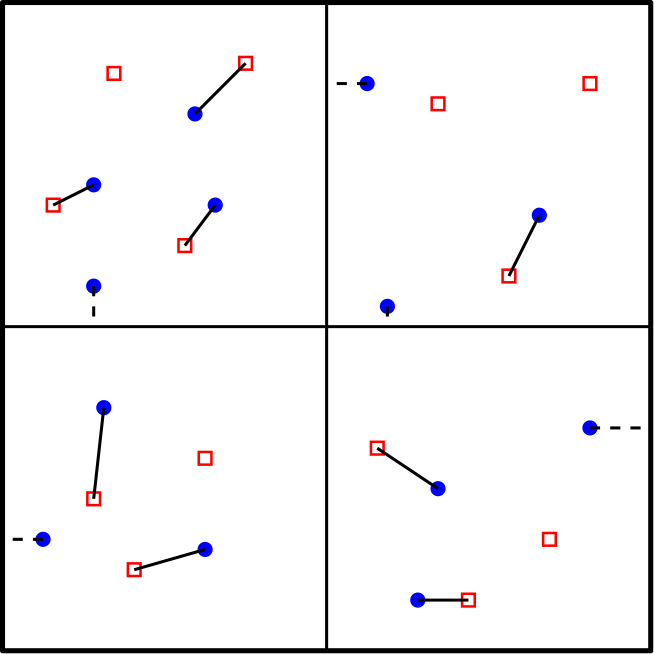
\includegraphics[width=0.32\linewidth]{figures/GRS1-new.png} \hspace{0.5em}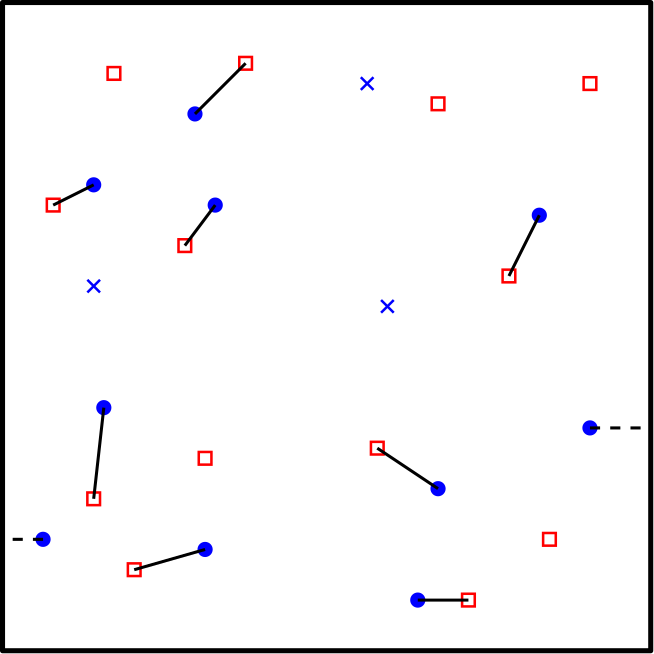
\includegraphics[width=0.32\linewidth]{figures/GRS2-new.png} \hspace{0.5em}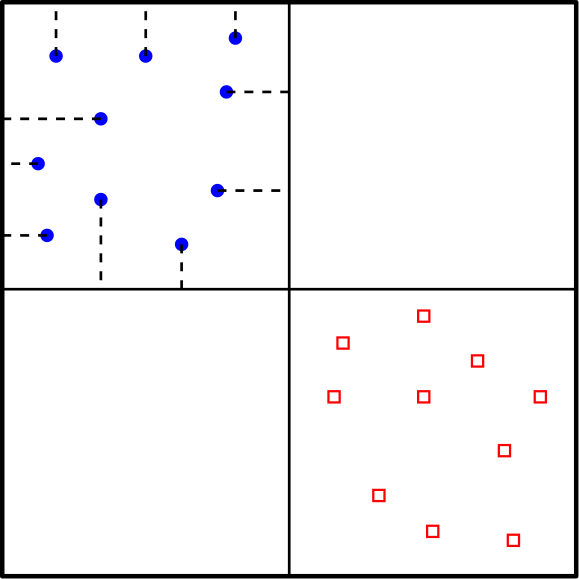
\includegraphics[width=0.32\linewidth]{figures/GRS-bad.png}
    \caption{Illustration of the GRS algorithm.}
    \label{fig:GRS}
\end{figure}

The GRS algorithm uses a (randomly-shifted) quadtree to divide the problem into smaller sub-problems. Within each square $\cell$ of the quadtree, their algorithm recursively computes a \emph{minimum-cost extended matching}, where each point of $B$ inside $\cell$ can either match to another point of $A$ inside $\cell$ or to the boundary of $\cell$ (Figure~\ref{fig:GRS}(left)). The algorithm combines minimum-cost extended matchings of the child squares by  \emph{erasing} their common boundary, freeing all points of $B$ that matched to this boundary (Figure~\ref{fig:GRS}(middle)), and iteratively matching the freed points. 

Interestingly, \citet{gattani2023robust} showed that when $A$ and $B$ are samples from the same distribution $\mu$, most points of $B$ will match to a close-by point in $A$, leaving only $\tilde{O}(n^{3/4})$ many points in $B$ matching to the boundary. Thus, erasing the common boundary only creates $\tilde{O}(n^{3/4})$ free points, each of which can be matched in $O(n\Phi(n))$ time, leading to an overall execution time of $\tilde{O}(n^{7/4}\Phi(n))$. However, this efficiency does not extend to arbitrary point sets. For instance, suppose all points of $A$ are in a child $\cell_1$ and all points of $B$ are in another child $\cell_2$. In this case, all edges of the minimum-cost matching cross the boundaries of $\cell_1$ and $\cell_2$. The minimum-cost extended matching at $\cell_2$, therefore, will match every point of $B$ to the boundary of $\cell_2$ (See Figure~\ref{fig:GRS}(right)). Erasing the common boundary between $\cell_1$ and $\cell_2$ creates $n$ free points, causing the conquer step to take $\Omega(n^2\Phi(n))$ time. Furthermore, unlike the Hungarian algorithm, the GRS algorithm does not guarantee the optimality of intermediate matchings. Therefore, it cannot be used to produce minimum-cost $t$-matchings. 


%Within each square of the quadtree, their algorithm recursively computes a \emph{constrained matching} where each point of $B$ can either matching to a point of $A$ or to the boundary of the square. The conquer step of the algorithm takes a constrained matching from the four children and computes a constrained matching at the parent. When $A$ and $B$ are a random partition of $U$, they used the fact that the

% For $d=2$, this results in a near-quadratic execution time. For higher dimensions, this is only slightly sub-cubic. 




%From Lemma~\ref{lem:spimatch}, the design of a sub-cubic algorithm for $n$-SPI will immediately lead to a sub-cubic algorithm for minimum-cost matching in a complete bipartite graph resolving a major open question in graph theory. Similarly, from Lemma~\ref{lem:}, design of algorithms for $n$-SPI that make sub-quadratic queries to the weighted nearest neighbor data structure will immediately lead to sub-quadratic algorithm for the geometric bipartite matching. 


%In contrast, Varadarajan~\cite{v_focs98} showed that finding a minimum-cost matching of size $n$ in a complete graph (not bipartite) on $2n$ points in $2$-dimensions can be done in $\tilde{O}(n^{3/2})$ time. 
%Figure~\ref{fig:matching} illustrates a difficult example for bipartite matching where two large subsets of $A$ (red points) and $B$ (blue points) are well-separated. Finding each edge of the optimal matching requires a search on the entire graph, requiring linear time per edge and quadratic time in total. In contrast, for the non-bipartite case, one can recursively solve the two clusters before merging these solutions by conducting a graph search on the entire graph.  

%\begin{figure}
%    \centering
%    \hspace{5em}
%    \includegraphics[width=0.3\textwidth]{figures/matching-bipartite.png}
%    \hfill
%    \includegraphics[width=0.3\textwidth]{figures/matching-non-1.png}
%    \hspace{5em}
%    \caption{(left) An instance of the bipartite matching problem in which, two large clusters of red and blue points (highlighted in the gray area) are well-separated and the majority of the optimal matching edges are between points in these clusters, and (right) the same point sets as an instance of the non-bipartite matching, where the majority of the optimal matching edges can be computed by recursively solving the clusters.}
%    \label{fig:matching}
%\end{figure}
%Despite this difficulty, there are two special cases of the Euclidean bipartite matching with real-valued edge costs for which there are sub-quadratic algorithms.
%First, Sharathkumar~\cite{s_socg13} showed that when the input is two-dimensional point sets with integer coordinates and Euclidean distances, one can compute the optimal matching in $O(n^{3/2}\Phi(n))$ time. Their algorithm uses an additive approximate solver to trap the edges of the optimal solution in a small planar subgraph of the complete bipartite graph. The correctness and efficiency analysis of their algorithm relies on the following facts: (a) the costs are the square root of integers, (b) the points are in the 2-dimensional plane, and (c) the Euclidean distance satisfies the triangle inequality. Thus, their result does not extend to points in $d$-dimensional space with real-valued coordinates. 

 
% For $\ell_2^q$ costs, sampling discrepancies cause the average cost of an edge in the optimal matching to increase. As a result, as $q$ increases, their analysis approaches the quadratic execution time.






% 

%Recently, Raghvendra and Sowle presented a primal-dual algorithm to maintain an offline optimal solution. Their algorithm will process each request in the arrival order and update the offline optimal by finding an ``augmenting trail" (a path where vertices may repeat). They show that these trails can be computed using a ``Hungarian search" style method in $O(n^2)$ time. Inspired by their algorithm, we present a very simple reduction from $k$-SPI and the $k$-SP problem to minimum-cost partial matching:


% Thus, finding the optimal solution to the $k$-SP and $k$-SPI problems can be done by computing the minimum-cost partial matching. In Section~\ref{}, we design a simple $O(n^2k)$ time algorithm to compute the minimum-cost partial matching.


%The problem of computing the minimum-cost matching in a complete bipartite graph between two sets $A$ and $B$ of $d$-dimensional points with $\ell_p$ costs is well-studied. Vaidya~\cite{vaidya1989geometry} showed that one can execute the Hungarian algorithm in $O(n^2\Phi(n))$ time, where $\Phi(n)$ is the query and update time of a weighted nearest neighbor data structure. For the $\ell_1$-norm and $d$-dimensions, he showed $\Phi(n)=O(\log^d n)$. For $d=2$ and the Euclidean norm, Vaidya~\cite{vaidya1989geometry} described a data structure with $\Phi(n)=O(\sqrt{n})$, which was subsequently improved to $\Phi(n)=\log^{O(1)}n$~\cite{kaplan2020dynamic}. Although the instances of minimum-cost matchings that are produced by $k$-SP and $k$-SPI are not complete graphs, we can adapt these implementations to find partial matchings in $O(nk\Phi(n))$ time. In fact, it 
 
% In the following, we establish a close connection between the $k$-SP (resp. $k$-SPI) problem and the geometric bipartite matching problem. 
 

% \subsection{Relating \texorpdfstring{$k$}{}-SP and \texorpdfstring{$k$}{}-SPI Problems to Geometric Bipartite Matching}
% We begin by showing that the $k$-SP (resp. $k$-SPI) can be reduced to solving an instance of geometric bipartite matching\footnote{Our reduction to the MCBM problem does not rely on geometry and extends to any cost function.}. Thus, $k$-SP and $k$-SPI problems can be solved optimally by simply using any geometric bipartite matching solver. \changed{Although this reduction has not been explicitly stated previously, there is an implicit connection between the dual formulation of the MCBM problem and the $k$-SPI problem, as explored by Raghvendra and Sowle~\cite{raghvendra2022scalable}. }   

% \myparagraph{Reducing $k$-SP and $k$-SPI to Geometric Bipartite Matching.} Given an input $\requests$ of requests to the $k$-SP problem, we construct a bipartite graph $\mathcal{G}_{\requests}$ with a vertex set $A\cup B$ and a set of edges $\mathcal{E}$ as follows. 
% {\it Vertex Set:} For each request $r_i$, we create a vertex $b_i$ (resp. $a_i$) in $B$ (resp. $A$) and  refer to it as the \emph{entry} (resp. \emph{exit}) gate for request $r_i$. 
% {\it Edge Set:} For any $a_i$ and every $j > i$, we connect the exit gate $a_i$ to the entry gate $b_j$ of request $r_j$ and assign it a cost $\distance{a_i}{b_j}:=\|r_i-r_j\|_p^q$. 
% It can be shown that a minimum-cost matching $M$ of size $(n-k)$ in $\mathcal{G}_\requests$ can be used to find an optimal solution to the $k$-SP problem. See Figure~\ref{fig:problem}.  The correctness proof of this reduction can be found in Appendix~\ref{sec:background}. 



% %\paragraph{Reducing $k$-SPI to Geometric Bipartite Matching:} 
% Similarly, given an input $\requests'=\eta\requests$ to the $k$-SPI problem, we construct a graph $\mathcal{G}_{\requests'}$ as follows.
% {\it Vertex Set:} For any server $j$ and its initial location $s_j$, we create a single vertex $a^j$ 
% % referred to as the exit gate 
% and add it to the set $A$. For each request $r_i$ in $\requests$, we create a vertex $b_i$ (resp. $a_i$) in $B$ (resp. $A$) and  refer to it as the entry (resp. exit) gate for $r_i$. 
% {\it Edge Set:} We connect every $a^j$ to all points $b_i\in B$ with an edge and assign it a cost $\distance{a^j}{b_i}:=\|s_j-r_i\|_p^q$. For any $r_i$ and every $j > i$, we connect the exit gate $a_i$ to the entry gate $b_j$ and assign it a cost $\distance{a_i}{b_j}:=\|r_i-r_j\|_p^q$. 
% Like in the case of $k$-SP, we show that a minimum-cost matching of size $n$ in $\mathcal{G}_{\requests'}$ can be converted to an optimal solution to the $k$-SPI problem. The details are provided in Appendix~\ref{sec:background}.


% \subsection{Related Work} 



%\myparagraph{$k$-SP and $k$-SPI related work.} For the $k$-SPI problem, Chrobak \textit{et al.}~\cite{chrobak1991new} presented a slightly different reduction to the minimum-cost flow of size $k$ on a weighted directed graph constructed as follows. In addition to the edges from exit gates to entry gates, they also add, for every request $r \in \requests$, an edge with a cost of $-\infty$ from its entry gate to the exit gate. They show how one can compute a flow of size $k$ in this network in $O(n^2k)$ time. There is substantial work on fast implementations of the $k$-SPI problem, especially in the context of online algorithms for the $k$-server and related problems; see for instance~\cite{raghvendra2022scalable,rudec2009fast,RUDEC20131004}.


%The $k$-SP and $k$-SPI problems are also closely related to a restricted version of the classical $k$ vehicle routing problem where each request has to be served at a pre-specified time\footnote{This problem is a special version of the $k$-vehicle routing problem with time windows.}.  Recently, Bertsimas \textit{et al.}~\cite{bertsimas2019k} found the optimal solutions to the vehicle routing problem with short time windows by solving a mixed integer program. For the special case where the time window is of length zero, i.e., a request has to be served at a pre-specified time, Bertsimas \textit{et al.}~\cite{bertsimas2019k} showed that the mixed integer program reduces to an instance of the minimum-cost flow problem.


  
 

%\todo{Do we need this?} Obtaining sub-quadratic algorithms for the minimum-cost bipartite matching for $2$-dimensional points with real-valued coordinates and $\ell_p^q$ costs remains a major open question in computational geometry. We note that, designing sub-quadratic algorithms for Euclidean bipartite matching for $d=\Omega(c^{\log^* n})$ is impossible under the orthogonal vectors conjecture~\cite{rohatgi}. There has also been extensive work on designing fast sub-quadratic approximations in geometric settings in both fixed and high dimensional space with applications in machine learning; see for instance~\cite{andoni2023sub, fox2022deterministic, lahn2021n, VaradarajanA99}


\myparagraph{Our results.} 
The optimal solutions to the $k$-SP (resp. $k$-SPI) problems can be computed in $\tilde{O}(nk\Phi(n))$ time by non-trivially adapting the Hungarian algorithm to find a minimum-cost $(n-k)$-matching (resp. $n$-matching) in $\mcG_{\requests}$ (resp. $\mcG_{\requests'}$). 
% The details of this algorithm are presented in Section~\ref{sec:nk-algod}.
However, it is worth noting that this algorithm still makes quadratic queries to the DWNN data structure when $k = \Theta(n)$. The main contribution of this paper is the design of a novel algorithm that, for any $k$, computes the optimal solution to the $k$-SP and $k$-SPI problems while making only a sub-quadratic number of queries to the DWNN data structure. 

%We provide a non-trivial adaptation of the Hungarian algorithm to compute a minimum-cost $(n-k)$-matching in $\mathcal{G}_{\requests}$ (resp. a minimum-cost $n$-matching in $\mathcal{G}_{\requests'}$) in $O(n^2k)$ time: Start from the solution to the $1$-SP problem, which is a minimum-cost $(n-1)$-matching in $\mcG_{\requests}$.  Iteratively reduce the matching size by $1$ by updating the matching along a minimum (negative) net-cost \emph{reverse augmenting path}, until the matching size becomes $n-k$.  The execution time of this algorithm can be improved to $\tilde{O}(nk\Phi(n))$ for edge costs that admit a DWNN data structure.

%For the $k$-SP (resp. $k$-SPI) problem, we present an algorithm that, given an input sequence $\requests$ (resp. $\requests'$), finds the optimal solution by solving the minimum-cost $(n-k)$-matching (resp. minimum-cost $n$-matching) in $\mathcal{G}_{\requests}$ (resp. $\mathcal{G}_{\requests'}$) by making sub-quadratic number of queries to the dynamic weighted nearest-neighbor data structure. 

\begin{theorem}\label{thm:kSP}
Given any sequence $\requests$ (resp. $\requests'=\servers\requests$) of $n$ requests (resp. $n$ requests and $k$ initial server locations) in $2$ dimensions with a spread of $\Delta$, and a value $1 \le k \le n$, there exists a deterministic algorithm that computes the optimal solution for the instance of $k$-SP (resp. $k$-SPI) problem under the $\ell_p$ norm in $\tilde{O}(\min\{nk, n^{1.8}\log \Delta\}\cdot\Phi(n))$ time.
\end{theorem}

Our algorithm also extends to higher dimensions, and for any dimension $d\ge 2$, it computes optimal solutions to the $k$-SP and $k$-SPI problems in $\tilde{O}(\min\{nk, n^{2-\frac{1}{2d+1}}\log \Delta\}\cdot\Phi(n))$ time (Theorem~\ref{thm:kSP-d} in Appendix~\ref{sec:appendix-high-d-ksp}). 
% Due to space limitations, we restrict the description of our algorithm and the analysis to the $k$-SP problem in $2$ dimensions. All other results including extension to higher dimensions and open questions are presented in the appendix.

% We also extend our algorithm to the $k$-SPI problem and present an algorithm that, given an input sequence $\requests'=\eta\requests$, finds the optimal solution by solving the minimum-cost maximum matching in  $\mathcal{G}_{\requests'}$. 

% \begin{theorem}\label{thm:kSPI}
% Given any input $\servers\sigma$ with a spread of $\Delta$ and $1 \le k \le n$ for the $k$-SPI problem, there exists a deterministic algorithm to compute the optimal solution for the instance that takes $\tilde{O}(\min\{nk, n^{1.8}\log \Delta\}\cdot\Phi(n))$ time.
% \end{theorem}


Developing algorithms for geometric bipartite matching that perform sub-quadratic queries to a DWNN data structure is a challenging task. Nevertheless, it follows from Theorem~\ref{thm:kSP} that the bipartite matching instances generated by $k$-SP and $k$-SPI problems (with bounded spread) can be solved by making sub-quadratic queries to a DWNN data structure. Solving instances with unbounded spread with sub-quadratic queries to DWNN, at least for the $k$-SPI problem, remains challenging. This is because, as established in Lemma~\ref{lemma:kSPI_reduction}, any such  
algorithm can find the $d$-dimensional minimum-cost bipartite matching algorithm under $\ell_1$ costs in sub-quadratic time.  

%In this paper, we present partitioning-based algorithms for $k$-SP and $k$-SPI problems that run in $\tilde{O}(n^{1.8}\Phi(n)\log \Delta)$ time.
%We also present an adaptation of the Hungarian algorithm with a running time of $\tilde{O}(nk\Phi(n))$. We establish Theorem~\ref{thm:kSP} by combining the two results.
%For the $k$-SP (resp. $k$-SPI) problem, our algorithms find the optimal solution by solving the minimum-cost $(n-k)$-matching (resp. maximum matching) in $\mathcal{G}_{\requests}$ (resp. $\mathcal{G}_{\requests'}$).
%Each iteration of the Hungarian algorithm computes a minimum-cost $(n-k)$-matching by initializing an empty matching $M$ and iteratively incrementing the matching size by augmenting $M$ along an augmenting path $P$ with the minimum net-cost, i.e., the path $P$ that results in the lowest increase in the matching cost.  

Our algorithm uses a hierarchical partitioning tree, whose nodes (referred to as cells) are axis-parallel rectangles with an aspect ratio of at most $3$. Each cell is divided into two smaller rectangles, forming its children. At any point during the execution of the algorithm, it maintains a set of \emph{current} cells $\mcC$ that partition the input points. It computes a minimum-cost extended $(n-k)$-matching where points of $B$ are allowed to match to the boundaries of these cells by repeatedly identifying a minimum net-cost augmenting path and augmenting the matching along this path.  Once a minimum-cost extended $(n-k)$-matching is computed, the algorithm removes a pair of sibling rectangles from the set of current cells and instead makes their parent cell current. By doing so, the common boundary between the siblings is erased, creating additional free points, which are then matched again by finding the minimum net-cost augmenting paths. When all the boundaries are erased, the algorithm terminates with the desired minimum-cost $(n-k)$-matching. 

There are three major hurdles in proving the efficiency of our algorithm. The first challenge is in finding a minimum net-cost augmenting path, which typically requires a search on the entire graph. However, for extended matchings, we show that the minimum net-cost augmenting path is fully contained inside one of the current cells.  This significantly improves efficiency, as the search can be limited to individual current cells, and the overall minimum can then be determined by selecting the path with the smallest net-cost among all current cells.
The second challenge is in bounding the time to merge two cells. Similar to the worst-case example for the GRS algorithm, the $k$-SP (or $k$-SPI) may have current cells with $\Theta(n)$ points, where the optimal solution matched each point of $B$ to a point of $A$ that is very far (see Figure~\ref{fig:ksp} (left)). Despite this, we show that any minimum-cost extended matching has only $O(n^{0.8})$ points that are matched to their common boundary, helping us in bounding the time required to merge cells. To establish this, we critically use the fact that every sub-problem has a hidden low-cost high-cardinality matching $M$ (with only sub-linearly many free points, see Figure~\ref{fig:ksp} (right)). 

The final challenge in the analysis is the following. The $k$ free points associated with the extended $(n-k)$-matching $M$ maintained by our algorithm may differ from the $k$ free points in the minimum-cost $(n-k)$ matching $M^*$. For instance, a point $b \in B$ may be free in $M^*$ but matched to the boundary in $M$, thereby leaving some other point $b'$ unmatched. Our algorithm corrects them via alternating and augmenting paths, each of which can take $\Theta(n)$ time to find. Since there can be $k$ such corrections, a na\"ive analysis leads to an upper bound of $O(nk)$. Surprisingly, by exploiting geometry, we show that the number of such corrections inside any current cell cannot exceed $O(n^{0.8})$. Using this observation, we bound the overall execution time of our algorithm by $\tilde{O}(n^{1.8}\Phi(n)\log \Delta)$.

%The optimal solution to the matching instance generated by the $k$-SP problem has $k$ free points in $A$ and $B$. During the execution of the algorithm, it is not clear how the $k$ free points of the optimal solution are distributed inside the various current cells. At an intermediate stage of the algorithm, suppose we incorrectly pick our $k$ free points to be inside a current cell $\cell$ with $\Theta(n)$ points; then, we are forced to correct it by matching these points (via $\Theta(k)$ searches) and instead making some other points free. This leads to an $\Omega(nk)$ execution time. We exploit geometry to show that surprisingly, after conducting $O(n^{0.8})$ such corrections inside a cell, it will no longer be current. This allows us to bound the overall execution time by $\tilde{O}(n^{1.8}\Phi(n)\log \Delta)$.


%We  the space into rectangles. Initially, each rectangle contains only one point each. 


%Next, our algorithm carefully combines two rectangles into a single one by erasing the common boundary between them. of the rectangular partition a

%We make several important observations that leads to an efficient algorithm. First, w  similar to Gattani~\etal\  we partition the space into rectangles where each rectangle initially contains only one point. We iteratively compute and allow for point to match with other points as well as the boundaries and compute an $(n-k)$  

%To improve the efficiency of the Hungarian algorithm, we define a new deterministic hierarchical partitioning tree to localize the search for augmenting paths. Each node of our hierarchical partitioning tree (referred to by cells) is a rectangle with an aspect ratio of at most $3$ and has at most two children. Our algorithm processes a set of \emph{current} cells that partition the input points and allows the points of $B$ to be matched to the boundaries of the cells. We show that all points of the minimum net-cost augmenting path will be fully inside one of the current cells. Thus, instead of conducting a global search for the augmenting path, we find this path by searching inside each cell and augmenting the matching along the path.  When we have a minimum-cost matching of size $(n-k)$, we identify two of the smallest sibling rectangles in the hierarchical partition and merge them making their parent current. Merging cells may create additional free points which are matched again by finding minimum net-cost augmenting paths. The algorithm stops with an optimal minimum-cost $(n-k)$ matching when all the boundaries are erased.  






% Unlike in the GRS algorithm where a randomly-shifted quadtree is used, we define a new deterministic hierarchical partitioning tree whose nodes are rectangles with an aspect ratio of at most $3$ and has at most two children. Our algorithm processes a set of \emph{current} cells that partition the input points. When the two sibling current cells are fully processed, we remove them from the current list, merge their solutions, and make their parent current. There are two major challenges in computing a minimum-cost $(n-k)$-matching in $\mathcal{G}_{\requests}$.

%First, similar to worst-case scenario in the Euclidean bipartite matching, there may be sub-problems in the $k$-SP (or $k$-SPI) with $\Theta(n)$ points, where the average cost of the optimal edges is comparable to the diameter (see Figure~\ref{fig:ksp} (left)) potentially making it expensive to merge the two rectangles.
%To overcome this difficulty, we observe that every sub-problem has a hidden low-cost high-cardinality matching $M$ (with only sub-linearly many free points). Using the existence of $M$, we show that for merging cells, there are only $O(n^{0.8})$ points that match to their common boundary. 

\begin{figure}
    \centering
    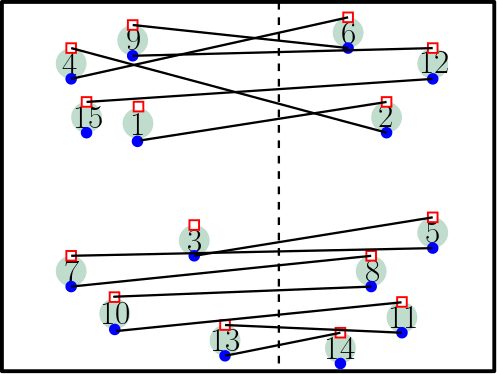
\includegraphics[width=0.45\textwidth]{figures/ours-bad1.png}
    \hspace{2em}
    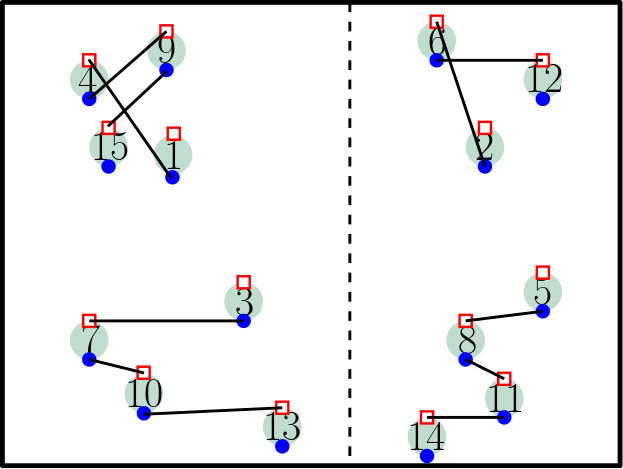
\includegraphics[width=0.45\textwidth]{figures/ours-bad2.png}
    \caption{(left) A sub-problem of the $k$-SP problem, where the optimal solution has a high cost, and (right) there exists a low-cost high-cardinality matching inside the sub-problems.}
    \label{fig:ksp}
\end{figure}


% (see Appendix~\ref{sec:nk-algod}). 
 

%To establish Theorem~\ref{thm:kSP}, consider the following adaptation of the Hungarian algorithm for solving the $k$-SP problem: Start from the solution to the $1$-SP problem, where a single server starts from the first request in $\sigma$ and serves all requests. Iteratively increment the number of servers by updating the matching along a minimum (negative) net-cost path that reduces the number of matching edges by one (referred to as the reverse augmenting path), until the matching size becomes $n-k$. 
%A fast implementation of this adaptation that uses a dynamic weighted nearest neighbor data structure runs in $\tilde{O}(nk\Phi(n))$ time. This approach also extends to the $k$-SPI problem straightforwardly. The details are presented in Appendix~\ref{sec:nk-algod}.

%Finally, the analysis in this paper can also be used to obtain better execution time of the GRS algorithm and we prove the following result:

Our proof techniques also improve the analysis of the GRS algorithm for the case where the cost between points $a \in A$ and $b \in B$ is given by $\|a-b\|_2^q$ for any $q \ge 2$. Previous work established that the GRS algorithm computes the minimum-cost perfect matching between two-dimensional stochastic points in $\tilde{O}(n^{2-\frac{1}{2(q+1)}}\Phi(n))$ time~\cite{gattani2023robust}. Notably, as $q$ approaches $\infty$, this analysis implies a quadratic number of queries to the DWNN data structure.
\citet{raghvendra2024new} recently observed that, for any $q\ge1$, there is a low-cost high-cardinality matching with only sub-linearly many free points between stochastic point sets. By incorporating this observation with the novel analysis techniques in our paper, we show that the GRS algorithm makes only a sub-quadratic number of queries to the DWNN data structure, regardless of the value of $q$. 
  
% Additionally, we generalize the analysis of the GRS algorithm to the setting in which we randomly partition $2n$ points to obtain the two sets $A$ and $B$ of $n$ points each. 

\begin{restatable}{theorem}{GRSAnalysis}\label{lemma:GRS-analysis}
    Suppose $U$ is a set of $2n$ points inside the unit square and $A$ is a subset chosen uniformly at random from all subsets of size $n$. Let $B=U\setminus A$.  Then, there exists an algorithm that computes the minimum-cost perfect matching on the complete bipartite graph on $A$ and $B$ under $\ell_2^q$ costs in $\tilde{O}(n^{7/4}\Phi(n)\log \Delta)$ expected time.
\end{restatable}

Note that the setting considered by \citet{gattani2023robust} in the analysis of the GRS algorithm, where the two sets $A$ and $B$ are i.i.d samples from the same distribution, is a special case of randomly partitioning a set of $2n$ points into two sets $A$ and $B$ of $n$ points, considered in Theorem~\ref{lemma:GRS-analysis}.


%We note that our analysis improves the execution time of the GRS algorithm for $q > 1$. As $q$ increases, the average cost of the edges in the optimal matching inside any sub-problem also increases. This results in a larger upper bound of $\tilde{O}(n^{2-\frac{1}{2(q+1)}}\Phi(n))$ based on the analysis in~\cite{gattani2023robust}. Using ideas similar to the ones in~\cite{raghvendra2024new}, we show that there is a high cardinality matching with a low cost between $A$ and $B$. Combining with an analysis similar to the one for $k$-SP, we obtain sub-quadratic bounds of Theorem~\ref{lemma:GRS-analysis}.

% \paragraph{Organization:} In the following, we present our algorithm for computing a minimum-cost $(n-k)$-partial matching in $\mathcal{G}_\sigma$ which corresponds to the optimal solution for $k$-SP problem. Our algorithm for $k$-SPI as well as the algorithm for bipartite matching on randomly colored points is simply obtained by setting $k=0$ in our algorithm for the $k$-SP problem. 


% \myparagraph{Organization.} \todo{Needs to be updated.} In Section~\ref{sec:geo-primal-dual}, we present our hierarchical partitioning and the primal-dual framework used by our algorithm. In Section~\ref{sec:k-seq}, we present our algorithm for computing a minimum-cost $(n-k)$-partial matching in $\mathcal{G}_\sigma$, which corresponds to the optimal solution for $k$-SP problem. In Section~\ref{sec:reduction}, we present our algorithm for the $k$-SPI and also show how any algorithm for $k$-SPI on points with arbitrary spread can be used to solve the Geometric Bipartite Matching Problem. The algorithm for bipartite matching on randomly colored points as well as its analysis is presented in Section~\ref{sec:randomly-colored}. In Section~\ref{sec:nk-algod}, we show how one can solve $k$-SP and $k$-SPI problems in $\tilde{O}(nk)$ time. We conclude in Section~\ref{sec:conclusion} by stating two important open questions. 



\paragraph{Organization.} In Section~\ref{sec:geo-primal-dual}, we establish our primal-dual framework for the minimum-cost bipartite matching problem and use it in Section~\ref{sec:k-seq} to present our sub-quadratic algorithms for the $k$-SP and $k$-SPI problems. We present our fast implementation of the Hungarian algorithm in Section~\ref{sec:nk-algod} and the improved analysis of the GRS algorithm in Section~\ref{sec:randomly-colored}. We conclude the paper by discussing some open questions in Section~\ref{sec:conclusion}.
